%% LaTeX2e class for student theses
%% sections/content.tex
%% 
%% Karlsruhe Institute of Technology
%% Institute of Information Security and Dependability (KASTEL)
%%
%% Template by
%% Dr.-Ing. Erik Burger
%% burger@kit.edu
%%
%% Adaption by
%% Annika Vielsack
%% vielsack@kit.edu
%%
%% Version 1.0, 2021-07-03
\definecolor{codegreen}{rgb}{0,0.6,0}
\definecolor{codegray}{rgb}{0.5,0.5,0.5}
\definecolor{codepurple}{rgb}{0.58,0,0.82}
\definecolor{backcolour}{rgb}{0.95,0.95,0.92}

\lstdefinestyle{mystyle}{
    backgroundcolor=\color{backcolour},   
    commentstyle=\color{codegreen},
    keywordstyle=\color{magenta},
    numberstyle=\tiny\color{codegray},
    stringstyle=\color{codepurple},
    basicstyle=\ttfamily\footnotesize,
    breakatwhitespace=false,         
    breaklines=true,                 
    captionpos=b,                    
    keepspaces=true,                 
    numbers=left,                    
    numbersep=5pt,                  
    showspaces=false,                
    showstringspaces=false,
    showtabs=false,                  
    tabsize=2
}

\lstset{style=mystyle}
\chapter{Preliminary Knowledge}
\label{ch:Backgroud}

\section{History}
\label{sec:Backgroud:History}


\section{Bitcoin}
\label{sec:Backgroud:Bitcoin}

\section{Ethereum}
\label{sec:Backgroud:Ethereum}

\section{Smart Contract}
\label{sec:Backgroud:SmartContracts}

\section{Security Analysis}
\label{sec:Backgroud:SecurityAnalysis}



\chapter{Most Common Vulnerabilities}
\label{ch:Vulnerabilities}

Presentation of what effected the smart contrats in the recent year.
The vulnerabilities that I found more often in papers that I read and I selected because I think they are the 
most rappresentative and the most common used by the attackers.

As introduction, I cite some papers that I read dealing with this topic. I select the following vulnerabilities, because I think they represent a risk still today.

\section{Race Codition}
\label{sec:Vulnerabilities:RaceCondition}
Race condition represents in computer science one of the most common vulnerabilities.
\citet{RaceConditionDef} identifies this as an even,  which occurs when two threads access a shared variable at the same time.
A case is illustruted when two threads read the value of a shared variable. After computing operations on that, they update the shared variable. The change applied by the last thread will be preserved and the other one will be lost.
In a Solidity context an analogous situation can happen. This can be exploited by attackers, for withrowing a higher amount of token or manipulating the price of it.

\citetitle{NotSoSmartContracts} is a repository that contains examples of common Ethereum smart contract vulnerabilities.
Vulnerable smart contracts and explanations are coupled and presented. I considered the smart contract \href{https://github.com/crytic/not-so-smart-contracts/blob/master/race_condition/RaceCondition.sol}{RaceCodition.sol} for showing a case of this class of vulnerability.
The vulnerability relies on the shared variable price, which is updated by the function changePrice (\autoref{lst:RaceCodition} line 15) and used by the function buy (\autoref{lst:RaceCodition} line 2).
\begin{lstlisting} [language={Solidity},caption={Cross-function RaceCondition vulnerable functions.}, label={lst:RaceCodition}]

    function buy(uint new_price) payable
        public
    {
        require(msg.value >= price);

        // we assume that the RaceCondition contract
        // has enough allowance
        token.transferFrom(msg.sender, owner, price);

        price = new_price;
        owner = msg.sender;
    }

    function changePrice(uint new_price){
        require(msg.sender == owner);
        price = new_price; 
    }    
\end{lstlisting}

When a user tries to buy tokens, the owner can call the function for changing the price of the token, consequently the attacked user will spend more than he expected.
 

\section{Denial Of Services}
\label{sec:Vulnerabilities:DOS}
The article \citet{CloudFareDos} of CloudFare, proposes a definition of denial-of-service (DoS) attack. It is a type of cyber attack in 
which an attacker aims to render a computer or a informatic service (logical or phisical) unavailable to its intended users by interrupting the 
device's normal functioning. 

In Solidity contetext, DoS consists of attacks where 
users can leave the contract inoperable for a small period of time, or in some cases, permanently.
It represents a cathegory of attacks, consequently it is not possible to classify a 
spefic vulnerability or methodology for exploiting a thread.

As an example of this class of attack, I selected the smart contract presented by \citet{Dos1}. 
It allows the user to place a bid to the contract. If it is the highest bid, it 
sends the previous leader the current bid and set the leader to the sender with the new highest bid.
The vulnerability relies on line 12 (\refname{lst:DosContract1}): the require condition is respected if the transaction which refunds the old leader doesn not revert. 
An attacker can exploit this vulnerability, creating a smart contract which cannot receive ether. Then it intacts with the vulnerable contract, becoming the leader.
When the vulnerable tries to refund the attacker one, it will always revert because it cannot receive ether and no one could become the new leader.

\begin{lstlisting} [language={Solidity},caption={Dos Vulnerable Contract.}, label={lst:DosContract1}]
    pragma solidity ^0.8.0;

    /**
     * @title VulnerableContract
     * @dev This contract is vulnerable to a denial of service (DoS) attack
     */
    contract VulnerableContract {
        address payable leader;
        uint256 public highestBid;
    
        function bid() external payable {
            require(msg.value > highestBid);
    
            // Refund the old leader, if it fails then revert
            require(leader.send(highestBid));
    
            leader = payable(msg.sender);
            highestBid = msg.value;
        }
    
        /// Helper function to check leader
        function getLeader() external view returns (address) {
            return leader;
        }
    }
    
\end{lstlisting}

\chapter{Real world Exploits}
\label{ch:Exploits}
Real-wolrd exploits that have happend in the recent years.


\section{Cover Protocol:Infinite Minting Exploit Nets Attacker \$4.4M }
\label{sec:Exploits:CoverProtocol}
On the 28th of December 2020, an exploit was abused on Cover Protocol's shield mining contract. 
The article shows the attackers could steal from project around \$ 4 million. 
The target of the attack was the smart contract \href{https://github.com/CoverProtocol/cover-token-mining/blob/main/contracts/Blacksmith.sol}{Blacksmith.sol}, its bug had the result to mint more rewards to the miner. 

\subsection{Cover Protocol}
\label{sec:CoverProtocol:Presentation}

\citet{CoverProtocol} interviewed Alan, the co-founder of the Cover Protocl. In his article he answers some question about his project, regarding its functionality and road map. 
It was an active protocol on the Ethereum blockchain; the developer deployed version 2,  because of the attack. 
Cover Protocol is a peer-to-peer coverage marketplace that utilizes ERC-20 fungible tokens to allow permissionless and non-KYC coverage. 
It can be described as a coverage provider.
The attack affected the rewards contract, consequently, the token's one even.  
The exploit can be classified under the name of "infinite mint".

\subsection{The exlpoit}
\label{sec:CoverProtocol:Exploit}
The develports's team reported \citep{CoverProtocolPostMortem} the technical analysis of the exploit the day after.
The contract containing the vulnerability is Blacksmith.sol. The core protocol was not affected, 
but the minting contract and the \$COVER token became unusable.
Firstly, the attackers created a new balancer liquidity pool for the target contract. The next step was to deposit token in it and execute the exploit, 
withdrawing funds from the contract thanks to a miscalculation of the rewards.
The bug relies on the misuse of two keywords in solidity: storage and memory. 

\paragraph{Memory} This keyword within Solidity allocates memory for a specific variable. 
In this instance, that variable is scoped to a specific function. 
The memory is cleared once the function has executed.

\paragraph{Storage} On the other hand this keyword within Solidity allows variables to act as a pointer into the storage of data in mappings or data structures. 
Storage data is persistent between function calls and transactions. 

The previous has a similar behave to the Random Access Memory (RAM) on a computing device, the latter stores into the persistent memory.

The vulnerable function is the deposit one.
\begin{lstlisting} [language={Solidity},caption={Deposit function.}, label={lst:coverdeposit}]
    function deposit(address _lpToken, uint256 _amount) external override {
        require(block.timestamp >= START_TIME , "Blacksmith: not started");
        require(_amount > 0, "Blacksmith: amount is 0");
        Pool memory pool = pools[_lpToken];
        require(pool.lastUpdatedAt > 0, "Blacksmith: pool does not exists");
        require(IERC20(_lpToken).balanceOf(msg.sender) >= _amount, "Blacksmith: insufficient balance");
        updatePool(_lpToken);

        Miner storage miner = miners[_lpToken][msg.sender];
        BonusToken memory bonusToken = bonusTokens[_lpToken];
        _claimCoverRewards(pool, miner);
        _claimBonus(bonusToken, miner);

        miner.amount = miner.amount.add(_amount);
        // update writeoff to match current acc rewards/bonus per token
        miner.rewardWriteoff = miner.amount.mul(pool.accRewardsPerToken).div(CAL_MULTIPLIER);
        miner.bonusWriteoff = miner.amount.mul(bonusToken.accBonusPerToken).div(CAL_MULTIPLIER);

        IERC20(_lpToken).safeTransferFrom(msg.sender, address(this), _amount);
        emit Deposit(msg.sender, _lpToken, _amount);
  }
\end{lstlisting}
At line 4 of \autoref{lst:coverdeposit}, the state of the pool is stored in a variable with the keyword memory. 
The function update \autoref{lst:coverupdate} is called, which updates the state of the pool. However, the variable pool, 
existing within the function, remains identical. 
\begin{lstlisting} [language={Solidity},caption={Update function.}, label={lst:coverupdate}]
    function deposit(address _lpToken, uint256 _amount) external override {
        require(block.timestamp >= START_TIME , "Blacksmith: not started");
        require(_amount > 0, "Blacksmith: amount is 0");
        Pool memory pool = pools[_lpToken];
        require(pool.lastUpdatedAt > 0, "Blacksmith: pool does not exists");
        require(IERC20(_lpToken).balanceOf(msg.sender) >= _amount, "Blacksmith: insufficient balance");
        updatePool(_lpToken);

        Miner storage miner = miners[_lpToken][msg.sender];
        BonusToken memory bonusToken = bonusTokens[_lpToken];
        _claimCoverRewards(pool, miner);
        _claimBonus(bonusToken, miner);

        miner.amount = miner.amount.add(_amount);
        // update writeoff to match current acc rewards/bonus per token
        miner.rewardWriteoff = miner.amount.mul(pool.accRewardsPerToken).div(CAL_MULTIPLIER);
        miner.bonusWriteoff = miner.amount.mul(bonusToken.accBonusPerToken).div(CAL_MULTIPLIER);

        IERC20(_lpToken).safeTransferFrom(msg.sender, address(this), _amount);
        emit Deposit(msg.sender, _lpToken, _amount);
  }
\end{lstlisting}

Then, deposit function at line 16 \autoref{lst:coverdeposit} estimates the reward per token updating the value of miner.rewardWriteoff, 
but it uses the wronge value of the parameter of pool.accRewardsPerToken.

Following the vulnerabilty, anyone can obtain an insane amount of minted tokens when they execute the claimRewards(address \_lpToken) function. 
This function, which is used to grab their rewards, ends up calling \_claimCoverRewards(Pool memory pool, Miner memory miner) which references the miner.rewardWriteoff. 
As that variable is much smaller than the actual pool.accRewardsPerToken, the contract results in minting an abundance of tokens.





\section{DeFi platform bZX: \$8M hack from one misplaced line of code}
\label{sec:Exploits:bZX}

\citet{bZxProtocol} explains how this protocl works. 
Anyone can use bZx to create apps that allow lenders, borrowers, and traders to interact with Ethereum based 
decentralised finance protocol.
It is a community-run project,moreover all major protocol changes requiring a community vote. 

Protocols can be deleveloped by bZx procol, an example is Fulcrum. 
It is a powerful DeFi platform for tokenized lending and margin trading. 
iTokens (margin loans) represent the earn holders interest on borrowed funds and pTokens (tokenized margin positions) allow your margin positions to be composable.

Unfortunately, it suffered a couple of attacks in February 2020.
The developrs explained the attackers could drain different currences,219,199.66 LINK, 4,502.70 Ether (ETH), 1,756,351.27 Tether (USDT), 
1,412,048.48 USD Coin (USDC) and 667,988.62 Dai (DAI): a total of \$8 millin in value. 
The arrack depends on a bug based on an incorrect sequence of operations.

The object of the attack was the contract named LoanTokenLogicStandard.
It implements the logic behind the protocol, for managing the borrows, loans and all the functionalities.
Every ERC20 token has a transferFrom() function, which has the aim to transfer the tokens.
Calling this function allowed the attacker to create and transfer an iToken to hitself: his balance could be artificially increased.
The duplicated tokens were then redeemed for their underlying collateral, 
with the hackers now “owning” a much higher percentage of the pool, so the attacker could withdraw the tokens.

The snipped code \autoref{lst:internalTransferFrom} shows the vulnerable function. 
The attacker called the function with the same amount of \_from and \_to. 
Since both addresses refer to the same one, line 27 decreases the balance of the address, but then line 31 increases the same balance. 
The problem relies on the estimating of the amount: it is the sum of the sent token and 
a variable (line 23), which stored the value of the balance before the transacion.

\begin{lstlisting} [language={Solidity},caption={Vulnerable function in LoanTokenLogicStandard contract.}, label={lst:internalTransferFrom}]
contract LoanTokenLogicStandard is AdvancedToken, GasTokenUser {
    using SafeMath for uint256;
    using SignedSafeMath for int256;

    modifier settlesInterest() {
        _settleInterest();
        _;
    }
    ... 
    function _internalTransferFrom(
        address _from,
        address _to,
        uint256 _value,
        uint256 _allowanceAmount)
        internal
        returns (bool)
    {
        if (_allowanceAmount != uint256(-1)) {
            allowed[_from][msg.sender] = _allowanceAmount.sub(_value, "14");
        }
        //Vulnerable lines 
        uint256 _balancesFrom = balances[_from];
        uint256 _balancesTo = balances[_to];

        require(_to != address(0), "15");

        uint256 _balancesFromNew = _balancesFrom
            .sub(_value, "16");
        balances[_from] = _balancesFromNew;

        uint256 _balancesToNew = _balancesTo
            .add(_value);
        balances[_to] = _balancesToNew;

        // handle checkpoint update
        uint256 _currentPrice = tokenPrice();

        _updateCheckpoints(
            _from,
            _balancesFrom,
            _balancesFromNew,
            _currentPrice
        );
        _updateCheckpoints(
            _to,
            _balancesTo,
            _balancesToNew,
            _currentPrice
        );

        emit Transfer(_from, _to, _value);
        return true;
    }
    ... 
\end{lstlisting}

The developers corrected the bug in few days. 
It was enough switching some line of code, in order to avoid the operations of sum and subtraction operate on the same balance. 
The code \autoref{lst:CorrectinternalTransferFrom} presents some differences. The operations regarding the receiver's balance are computed (lines 13-15), then those which deal with the sender's one (16-20).
\begin{lstlisting} [language={Solidity},caption={Corrected bug in LoanTokenLogicStandard contract.}, label={lst:CorrectinternalTransferFrom}]
    function _internalTransferFrom(
        address _from,
        address _to,
        uint256 _value,
        uint256 _allowanceAmount)
        internal
        returns (bool)
    {
        if (_allowanceAmount != uint256(-1)) {
            allowed[_from][msg.sender] = _allowanceAmount.sub(_value, "14");
        }
        require(_to != address(0), "15");
        uint256 _balancesFrom = balances[_from];
        uint256 _balancesFromNew = _balancesFrom
            .sub(_value, "16");
        balances[_from] = _balancesFromNew;
        uint256 _balancesTo = balances[_to];
        uint256 _balancesToNew = _balancesTo
            .add(_value);
        balances[_to] = _balancesToNew;
        // handle checkpoint update
        uint256 _currentPrice = tokenPrice();
        _updateCheckpoints(
            _from,
            _balancesFrom,
            _balancesFromNew,
            _currentPrice
        );
        _updateCheckpoints(
            _to,
            _balancesTo,
            _balancesToNew,
            _currentPrice
        );
        emit Transfer(_from, _to, _value);
        return true;
    }   
\end{lstlisting}


\section{XSURGE on BSC Chain}
\label{sec:Exploits:XSURGE}

The \citet{XSurgeWeb}'s whitepaper provides a presentation of the ecosystem.
It is described as a great DeFi investing idea based on proprietary pricing algorithms embedded in the Surge Token Variants' contracts.
Surge Token Variants each have their own Market Maker, allowing them to trade continuously and outlast both 
centralised and decentralised exchanges. 
The strategy is to reward long-term holding by increasing a
holder's claim of the backing asset. Each Surge Token utilizes a built-in contract exchange system that renounces the need for
a traditional liquidity pool. Both assets are stored within the contract itself, 
rather than a liquidity pool pair of the backing asset to the
token using a traditional market maker method for exchange and price calculation.

One of the Surge Token is SurgeBNB, the one which is my focus of analysis.
\citet{XSurgeBNB} explains in deep how the attack to this contract occured. 
The Official claimed that the attacker had stolen \$5 million in SurgeBNB through a backdoor vulnerability.
XSURGE stated that a potential security vulnerability in the SurgeBNB contract was discovered on August 16th.

The attack is mabe by 4 main steps:
\begin{enumerate}
    \item the attacker borrow  10,000BNB through flash loans.
    \item Use all the BNB to buy SURGE. According to the current price, 
    the attacker can buy 1,896,594,328,449,690 SURGE
    \item He calls the "sell" function, for selling the obtained SURGE.
    \item The sale function alters the data after the transfer, and the transfer code has a reentrance vulnerability.
    When the attack contract acquires BNB, the period before the SURGE contract's state changes 
    (\refname{lst:SellSURGE} line 15 ), the attack contract can use the reentrance 
    vulnerability to purchase SURGE again.
\end{enumerate}

\begin{lstlisting} [language={Solidity},caption={Sell function of Surge (SURGE) token.}, label={lst:SellSURGE}]
    function sell(uint256 tokenAmount) public nonReentrant returns (bool) {
        
        address seller = msg.sender;
        
        // make sure seller has this balance
        require(_balances[seller] >= tokenAmount, 'cannot sell above token amount');
        
        // calculate the sell fee from this transaction
        uint256 tokensToSwap = tokenAmount.mul(sellFee).div(10**2);
        
        // how much BNB are these tokens worth?
        uint256 amountBNB = tokensToSwap.mul(calculatePrice());
        
        // send BNB to Seller
        (bool successful,) = payable(seller).call{value: amountBNB, gas: 40000}(""); 
        if (successful) {
            // subtract full amount from sender
            _balances[seller] = _balances[seller].sub(tokenAmount, 'sender does not have this amount to sell');
            // if successful, remove tokens from supply
            _totalSupply = _totalSupply.sub(tokenAmount);
        } else {
            revert();
        }
        emit Transfer(seller, address(this), tokenAmount);
        return true;
    }
\end{lstlisting}


The bnb Amount of the contract stays intact, and the total amount of SURGE tokens \texttt{ totalSupply }  
has not been updated, because the attack contract spends all of the BNB balance to acquire SURGE
 each time (still remains the quantity before the sell).
As a result, the price of token falls, allowing the attacker to purchase additional SURGE. 


\begin{lstlisting} [language={Solidity},caption={Purchase function of Surge (SURGE) token.}, label={lst:SellPurchase}]
    function purchase(address buyer, uint256 bnbAmount) internal returns (bool) {
        // make sure we don't buy more than the bnb in this contract
        require(bnbAmount <= address(this).balance, 'purchase not included in balance');
        // previous amount of BNB before we received any        
        uint256 prevBNBAmount = (address(this).balance).sub(bnbAmount);
        // if this is the first purchase, use current balance
        prevBNBAmount = prevBNBAmount == 0 ? address(this).balance : prevBNBAmount;
        // find the number of tokens we should mint to keep up with the current price
        uint256 nShouldPurchase = hyperInflatePrice ? _totalSupply.mul(bnbAmount).div(address(this).balance) : _totalSupply.mul(bnbAmount).div(prevBNBAmount);
        // apply our spread to tokens to inflate price relative to total supply
        uint256 tokensToSend = nShouldPurchase.mul(spreadDivisor).div(10**2);
        // revert if under 1
        if (tokensToSend < 1) {
            revert('Must Buy More Than One Surge');
        }
        
        // mint the tokens we need to the buyer
        mint(buyer, tokensToSend);
        emit Transfer(address(this), buyer, tokensToSend);
        return true;
    }
\end{lstlisting}

Repeating three times of Round 2 and Round 3 , the attacker accumulates a large amount of SURGE through reentry, and then sells all the SURGE to make a profit.

At the end of this transaction, the attack contract sold 1,864,120,345,279,610,000 SURGE, 
obtained 10327 BNB, and finally the profitable 297 BNB was sent to the attacker's address.

The following are the modifications suggested by the Beosin technical team for this attack:
\begin{itemize}
    \item any transfer operation should be place after the state changes to avoid reentry assaults.
    \item Instead of using "call. value," use transfer or send to transfer. 
\end{itemize}

\section{CBDAO: an example of rug pull}
\label{sec:Exploits:CBDAO}
Developers should watch out for possible attacks. They should audit and test their contract to find possible vulnerabilities and apply patches.
In the decentralized finance context, even the investors should worry about malicious developers, who convince the investors to invest and then steal their investments.
These class of fraud are basically  type of exit scam and decentralized finance (DeFi) exploit, it is classified with the name of rug pull.


\citet{RugPullDef} defines rug pull as a  type of crypto scam that occurs when a team pumps their project's token before disappearing with the funds, 
leaving their investors with a valueless asset. 
Fraudulent developers create a new crypto token, 
pump up the price and then pull as much value out of them as possible before abandoning them as their price drops to zero.

An example of this type of fraud is the one presented in the article \citet{CBDAO}.
It seems the malicious developers could steal around 1 million dollar in ethereum (ETH). 

The project main token was \$BREE. For attracting ealry investors, they associeted to it a presale token, named \$SBREE. 
The ones who bought that, could swap their amount of presale token in \$BREE once the token was published, having an advantage.
Unfortubatly, one of the admin wallets exploited a backdoor in the SBREE token contract, minted 50,000 SBREE. After that, the attacker soled that amount in BREE token and sold it on the market.
That pushed down the price of BREE at the expense of other holders. The 50,000 BREE was sold for under 200 ETH.

Following the operation of the \href{https://etherscan.io/address/0x85c90f369676789d3234ecf07adb5262df1bcf15#tokentxns}{malicious developer}, it is possible to understand how the fraud occured.
\href{https://etherscan.io/tx/0x3bf7b06d6737e6d222234acc58dea634c7ff75e6cc447bece6cc264f2e1db9d2}{This transacion}, achieved by etherscan, shows the attacker called the mint function and could generate 
50.000 SBREE. After that, it called the \href{https://etherscan.io/address/0x60c3094a586b02cb416ec4df31119d4513ff0dde#code}{BreePurchase} 
contract for swapping the token in BREE and then swap those in ETH on Uniswap.

The backdoor relies on the malicious management of access control. The admin, with the function grantRole, allow another wallet to be the Minter, so it called the function mint.
\begin{lstlisting} [language=Solidity, caption={Backdoor inside the contract}, label={lst:SBREE}]
    
    ... 
    function _grantRole(bytes32 role, address account) private {
        if (_roles[role].members.add(account)) {
            emit RoleGranted(role, account, _msgSender());
        }
    }
    ... 


    contract Roles is AccessControl {

    bytes32 public constant MINTER_ROLE = keccak256("MINTER");
    bytes32 public constant OPERATOR_ROLE = keccak256("OPERATOR");

    constructor () public {
        _setupRole(DEFAULT_ADMIN_ROLE, _msgSender());
        _setupRole(MINTER_ROLE, _msgSender());
        _setupRole(OPERATOR_ROLE, _msgSender());
    }

    modifier onlyMinter() {
        require(hasRole(MINTER_ROLE, _msgSender()), "Roles: caller does not have the MINTER role");
        _;
    }

    modifier onlyOperator() {
        require(hasRole(OPERATOR_ROLE, _msgSender()), "Roles: caller does not have the OPERATOR role");
        _;
    }
}

//the contract inherit Roles contetract
    ... 
    modifier onlyMinter() {
        require(hasRole(MINTER_ROLE, _msgSender()), "Roles: caller does not have the MINTER role");
        _;
    }
    ... 
    function _mint(address account, uint256 amount) internal virtual {
        require(account != address(0), "ERC20: mint to the zero address");

        _beforeTokenTransfer(address(0), account, amount);

        _totalSupply = _totalSupply.add(amount);
        _balances[account] = _balances[account].add(amount);
        emit Transfer(address(0), account, amount);
    }
    ... 


\end{lstlisting} 
    

\chapter{Analysis Tools}
\label{ch:Tools}
In this chapter I describe the tools and their capabilities, how they perform the Analysis.

\section{Typologies of Tools}
\label{sec:Tools:Typologies}
I explain the different types of analysis exsting in general, as Symbolic execution, formal specification, scanner, Symbolic execution.

\section{Tools for analysing properties specified by user}
\label{sec:Tools:Specification}
Description of Different types of tool, like a taxonomy.

Description of tools that we are going to use. 
I would say like an overview of their papaer.

\subsection{Celestial}
\label{sec:Specification:Celestial}


\subsection{SmartPulse}
\label{sec:Specification:SmartPulse}

\subsection{VeriSol}
\label{sec:Specification:VeriSol}


\subsection{Echidna}
\label{sec:Specification:Echidna}
Echidna is an open-source smart contract fuzzer, developed by \citet{Echidna}, which makes it easy to automatically generate tests to detect violations in
assertions and custom properties.
Rather than relying on a fixed set of pre-defined bug oracles to detect vulnerabilities
during fuzzing campaigns, Echidna supports three types of proper-
ties: 
\begin{itemize}
    \item user-defined properties (for property-based testing;
    \item assertion checking;
    \item gas use estimation.
\end{itemize}

Figure \autoref{fig:echdina_architecture} depicts the Echidna architecture as a two-step process: pre-processing and fuzzing.
The tool starts with a collection of contracts that have been supplied, as well as attributes that have been integrated into one of the contracts.
Echidna uses Slither , smart contract static analysis framework presenet in \autoref{sec:WithoutSpecification:Slither}, to build and analyse the contracts in order to find relevant constants and functions that directly handle Ether (ETH).
The fuzzing effort begins in the second stage. 
Using the application binary interface (ABI) given by the contract, significant constants stated in the contract, 
and any previously gathered sets of transactions from the corpus, this iterative procedure creates random transactions. 
When a property violation is detected, a counterexample is created to indicate the smallest and most basic sequence of operations that caused the failure. 

\begin{figure}
    \centering
    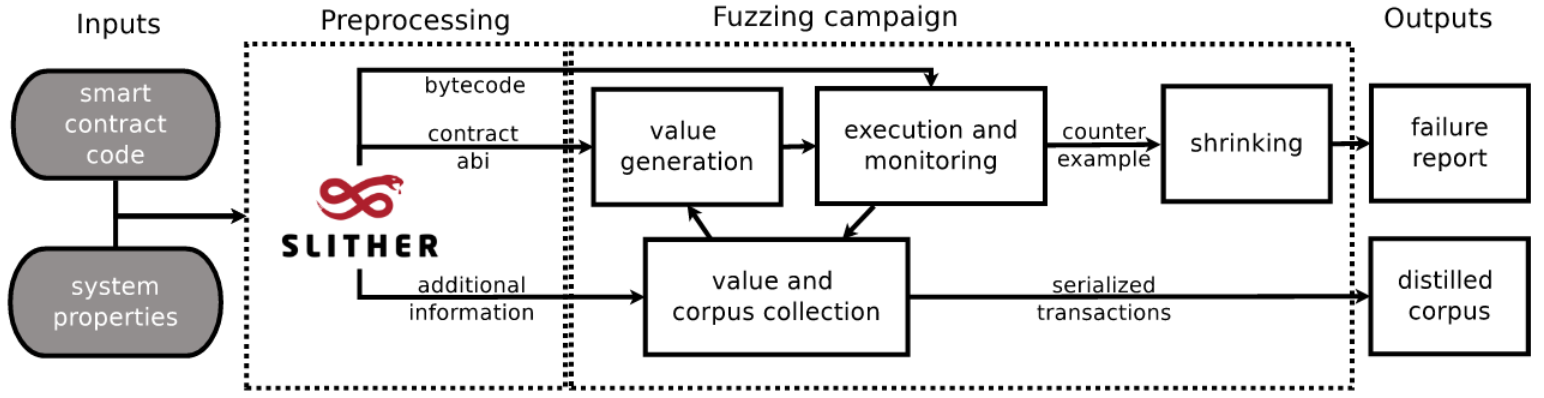
\includegraphics[width=10cm]{logos/echidna.png}
    \caption{Echidna architecture}
    \label{fig:echdina_architecture}
\end{figure}

The code \autoref{lst:EchidnaCode} provides an example of invariant in Echdina context. The Solidity contract contains a vulnerability a the backdoor function. The output of the terminal is presented in Listing \autoref{lst:EchidnaResult}: the attacker. For breaking the property, can call in order the tunctions airdrops() and backdoor()

\begin{lstlisting} [language=Solidity, caption={Solidity smart contract implementing a vulnerable Token and an Echidna invariant function.}, label={lst:EchidnaCode}]
contract Token{
    mapping(address => uint) public balances;
    function airdrop() public{
        balances[msg.sender] = 1000;
    }
    function consume() public{
        require(balances[msg.sender]>0);
        balances[msg.sender] -= 1;
    }
    function backdoor() public{
        balances[msg.sender] += 1;
    }
    function echidna_balance_under_1000() public view returns(bool){
        return balances[msg.sender] <= 1000;
    }
}
\end{lstlisting}
\begin{lstlisting} [caption={Tool's result after the execution of the precious code.}, label={lst:EchidnaResult}]
    $ echidna-test testtoken.sol --contract TestToken
    ...
    echidna_balance_under_1000: failed!
    Call sequence, shrinking (1205/5000):
    airdrop()
    backdoor()

    ...
\end{lstlisting}

The tool can be even used to test assertions. 
The aim is equivalent of the invariant testing methodology, 
but in this case properties are expressed using the Solidity annotation of assertion.

\subsection{Solc-Verify}
\label{sec:Specification:Solc-Verify}

\citet{SolcVerify} present solc-verify, a source-level verification tool for
Ethereum smart contracts. It takes smart contracts written
in Solidity and discharges verification conditions using modular program
analysis. It is built on top of the Solidity compiler, so it reasons at the level of the contract source code. 
Becuase of that, Solc-verify is able to reason about high-level contract attributes 
while accurately modeling low-level language semantics.

Solc-verify is implemented as an extension to the Solidity compiler.
It accepts a collection of Solidity contracts, including specification annotations, and uses 
the Boogie verifier and SMT solvers to discharge verification conditions. 

As \citet{SolcVerify_2} explain, Solc-verify translates the annotated contracts to the Boogie Intermediate Verification
Language (IVL). The key idea of the translation is to encode state variables as global heaps
and functions as procedures. Solc-verify relies on the Boogie verifier to perform modular
verification by discharging verification conditions to SMT solvers. The verification conditions
encode the function body while assuming the preconditions, and then check if postconditions
hold. In this process, function calls are replaced by their specification and loops by their
invariants (modularity). Finally, the results are back-annotated to the Solidity source.

\autoref{lst:SimpleBank} present an example of annotation, which states that the contract will ensure
that the sum of individual balances is equal to the total balance in the bank.


\begin{lstlisting} [language=Solidity, caption={An example Solidity smart contract implementing a simple bank with SolcVerify annotations.}, label={lst:SimpleBank}]
pragma solidity >=0.7.0;

/**
 * @notice invariant __verifier_sum_uint(balances) <= address(this).balance
 */
contract SimpleBank {
    mapping(address=>uint) balances;

    function deposit() public payable {
        balances[msg.sender] += msg.value;
    }

    function withdraw(uint256 amount) public {
        require(balances[msg.sender] > amount);
        bool ok;
        (ok, ) = msg.sender.call{value: amount}(""); // Reentrancy attack
        if (!ok) revert();
        balances[msg.sender] -= amount;
    }
}
\end{lstlisting}




\citet{SolcVerify_3} on GitHub repository, present the specification annotations. Those must be included in special documentation comments (/// or /** */) and must start with the special doctag @notice. 
They must be side-effect free Solidity expressions (with some verifier specific extensions) and can refer to variables within the scope of the annotated element. Functions cannot be called in the annotations, except for getters.
The currently available annotations are listed below. 

\begin{itemize}
    \item Function pre/postconditions can be attached to functions. Preconditions are assumed before executing the function and postconditions are checked (asserted) in the end. The expression can refer to variables in the scope of the function. The postcondition can also refer to the return value if it is named.
    \item Contract level invariants can be attached to contracts. They are included as both a pre- and a postcondition for each public function. The expression can refer to state variables in the contract (and its balance).
    \item Loop invariants can be attached to for and while loops. The expression can refer to variables in scope of the loop, including the loop counter.
    \item Modification specifiers can be attached to functions. The target can be a (1) state variable, including index and member accesses or (2) a balance of an address in scope. Note however, that balance changes due to gas cost or miner rewards are currently not modeled.
    \item Event data specification can be attached to events that should be emitted when certain data changes. 
    Events can declare the state variable(s) they track for changes, or in other words, the variables for which the event should be emitted on a change.
\end{itemize}

\section{Tools without specification}
\label{sec:Tools:WithoutSpecification}

\subsection{VeriSmart}
\label{sec:WithoutSpecification:VeriSmart}

\subsection{SmartTest}
\label{sec:WithoutSpecification:SmartTest}

SmartTest is a safety analayzer for Ethereum smart contracts develeoped by \citet{SmarTest}. 
It adopts a symbolic execution technique for effectively detecting vulnerable transaction sequences. 
The main challenge of the project involves the tool to find transaction sequences,
revealing the vulnerabilities of the analysed smart contract. Therefore, bugs are discoved as the cause of the interaction of multiple transactions.
The purpose of SmartTest is to automatically deliver vulnerable transaction sequences, 
which demostrate the weaknesses of the smart contract.
The main idea is to build a statistical model using known vulnerable transaction sequences and use it to direct symbolic execution toward 
more successfully detecting unknown vulnerabilities. 
Symbolic execution is guided by statistical language models, so it can prioritize transacion sequences which are likely to reveal vulenrablities.
This statregy involves firstly to run unguided symbolic
execution on existing vulnerable contracts, then to learn a probablity distribution over vulnerable transaction sequences.

The tool is implemented as an extension of VeriSmart \autoref{sec:WithoutSpecification:VeriSmart}.
SmartTest is build on top of that, adding its own functionalities:
\begin{itemize}
    \item symbolic execution with a language model.
    \item Symbolic executor for transaction sequences.
    \item Constraint solving optimization.
\end{itemize}
The installation of VeriSmart is necessary for running the tool. After that, the command \autoref{lst:SmarTestRun} is run for using VeriSmart in SmarTest mode.
\begin{lstlisting} [caption={SmarTest Command.}, label={lst:SmarTestRun}]
    ./main.native -input examples/leak_unsafe.sol -mode exploit -exploit_timeout 10
\end{lstlisting}

The report \autoref{lst:SmarTestReport} shows an example of output of SmarTest, which provides the sequence of funtions for exploiting the found bug.
\begin{lstlisting} [caption={SmarTest Example Report.}, label={lst:SmarTestReport}]
    [5] [IO] line 39, (balance[_to] + _value) : disproven, 14.528264s
    1: Example
       {}
       {msg.sender: #x0000000000000000000000000000000000010000,
        msg.value: 0}
    2: approve
       {_spender: #x0000200000000000000000000000000000000000,
        _value: 44365792925664701906080996193724747326645573793336555789802397725137091694592}
       {msg.sender: #x0000000000000000001000000000000000000000,
        msg.value: 0}
    3: mintToken
       {_target: #x0000000000000000001000000000000000000000,
        _amount: 87371285831589357636669861644764241805818792173739087408632338890371299803136}
       {msg.sender: #x0000000000000000000000000000000000010000,
        msg.value: 0}
    4: transferFrom
       {_from: #x0000000000000000001000000000000000000000,
        _to: #x0000000000000000001000000000000000000000,
        _value: 44365787749354941813158155617657849918564739183862151684054205258595743830016}
       {msg.sender: #x0000200000000000000000000000000000000000,
        msg.value: 0}

\end{lstlisting}

The detection of  the following six types of security-critical vulnerabilities are supported by the tool: integer over/underflow, 
assertion violation, division-by-zero, 
ERC20 standard violation, Ether-leaking vulnerability (e.g., 
unauthorized access to transfer), and suicidal vulnerability 
(e.g., unauthorized access to selfdestruct).
In the paper, the authors  focus on just those, without considering vulnerabilities that require analysis of
the interaction of multiple contracts to demonstrate the flaws 
(e.g., reentrancy).





\subsection{Slither}
\label{sec:WithoutSpecification:Slither}
Slither is described by \citet{Slither} as an open-source static analysis framework.
It uses its own intermediate representation, SlithIR, which was created to simplify static analysis of Solidity code. 
Concolic analysis, taint analysis, and control flow checking are involved for detecting a variety
of security vulnerabilities. It is designed to provide
granular information about smart contract code and the flexibility necessary to support many applications.

It is mainly used for:
\begin{itemize}
    \item Automated vulnerability detection: a large variety of
    smart contract bugs can be detected without user inter-
    vention.
    \item Automated optimization detection: Slither detects code
    optimizations that the compiler misses.
    \item Code understanding: printers summarize and display
    contracts' information to aid in the study of the codebase.
    \item Assisted code review: through its API, a user can interact
    with Slither.
\end{itemize}

Slither implements more than twenty bug detectors, regarding reetrancy, Uninitialized variables,
Shadowing and many other. The tool allows the developers to integrate more detectors, therefore it extends Slither's capabilities
to detect more advanced bugs.

\citet{SlitherGitHub} is written in python 3 and it is published on GitHub.
During the installation, I did not find any particular issues.

\subsection{Mythril}
\label{sec:WithoutSpecification:Mythril}
Mythril is a security analysis tool for Ethereum smart contracts. It was introduced by \citet{Mythril}.

The tool  relies on concolic analysis, taint analysis and control flow checking of the EVM bytecode to
prune the search space and to look for values that allow exploiting
vulnerabilities in the smart contract.
It is targeted at finding common vulnerabilities, 
and is not able to discover issues in the business logic of an application. \citet{SWCRegistry}'s taxonomy of vulnerabilities is used by Mythril for classify them. 
Listig \autoref{lst:MythrilOutput} illustrates an example of output of Mythril analysis. 
At the secocond line, there is the reference to the vulnerability classified by SWC Registry with the ID of 110 (Assert Violation).


\begin{lstlisting} [caption={Example of the output of Mythril Analysis.}, label={lst:MythrilOutput}]
==== Exception State ====
SWC ID: 110
Severity: Medium
Contract: Token
Function name: transferArray(address[],uint256[])
PC address: 4385
Estimated Gas Usage: 944 - 6585
An assertion violation was triggered.
It is possible to trigger an assertion violation. Note that Solidity assert() statements should only be used to check invariants. Review the transaction trace generated for this issue and either make sure your program logic is correct, or use require() instead of assert() if your goal is to constrain user inputs or enforce preconditions. Remember to validate inputs from both callers (for instance, via passed arguments) and callees (for instance, via return values).
--------------------
In file: test.sol:309

function transferArray(address[] tos, uint256[] values) public returns (bool) {
        for (uint8 i = 0; i < tos.length; i++) {
            require(transfer(tos[i], values[i]));
        }

        return true;
    }

--------------------

\end{lstlisting}

\subsection{Maian}
\label{sec:WithoutSpecification:Maian}

\subsection{Securify}
\label{sec:WithoutSpecification:Securify}

\subsection{ContractLarva}
\label{sec:WithoutSpecification:ContractLarva}
contractLarva is a runtime verification tool for Solidity contracts. 

\chapter{Results of testing}
\label{ch:Results}
